\documentclass{article}
\usepackage[paperwidth=24cm,paperheight=14cm,margin=0.5cm]{geometry}
\usepackage{tikz}
\usepackage{xcolor}

\begin{document}
\pagestyle{empty}

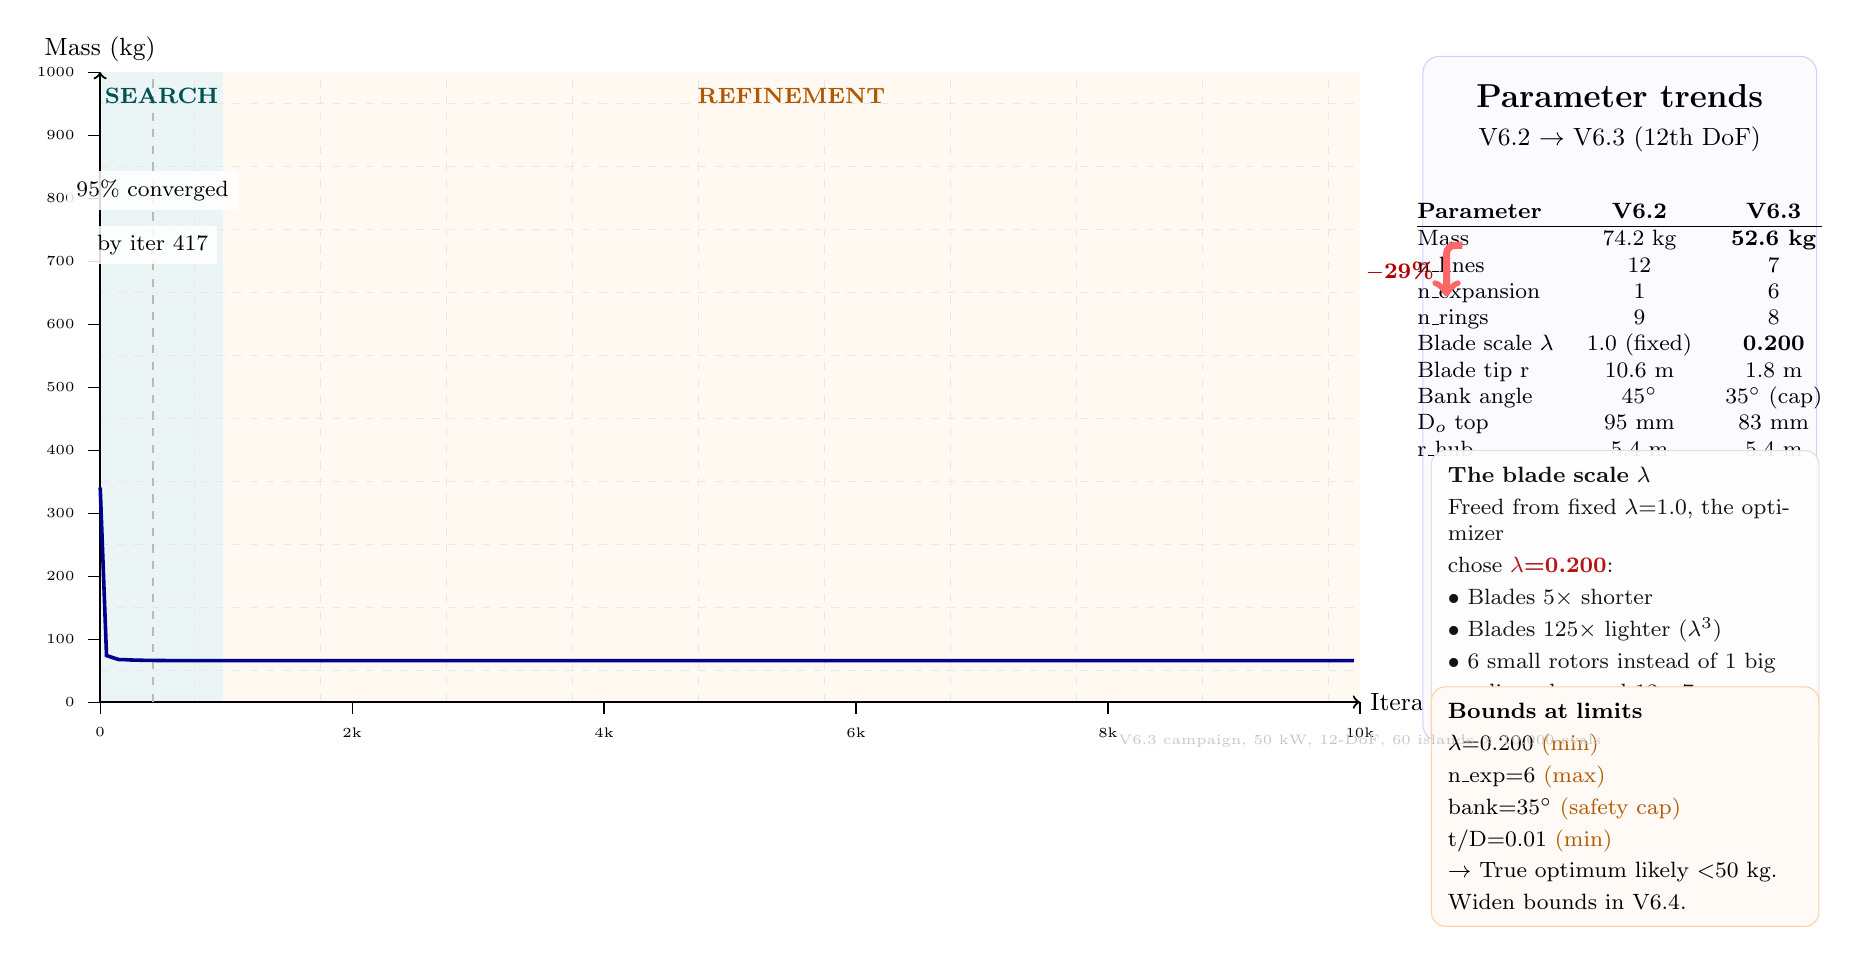
\begin{tikzpicture}[scale=1.0]

% --- BACKGROUNDS ---
\fill[teal!8] (2.0,2.0) rectangle (3.56,10.0);
\fill[orange!5] (3.56,2.0) rectangle (18.0,10.0);

% Grid
\draw[gray!18, very thin, dashed] (2.0,2.0) grid[xstep=1.6,ystep=0.8] (18.0,10.0);

% Axes
\draw[thick, ->] (2.0,2.0) -- (18.0,2.0) node[right, font=\small] {Iteration};
\draw[thick, ->] (2.0,2.0) -- (2.0,10.0) node[above, font=\small] {Mass (kg)};

% Y ticks
\foreach \y/\l in {2.0/0, 2.8/100, 3.6/200, 4.4/300, 5.2/400, 6.0/500, 6.8/600, 7.6/700, 8.4/800, 9.2/900, 10.0/1000} {
  \draw (1.85,\y) -- (2.0,\y); \node[left, font=\tiny] at (1.8,\y) {\l};
}
% X ticks
\foreach \x/\l in {2.0/0, 5.2/2k, 8.4/4k, 11.6/6k, 14.8/8k, 18.0/10k} {
  \draw (\x,1.85) -- (\x,2.0); \node[below, font=\tiny] at (\x,1.8) {\l};
}

% Phase boundary at iter 417
\draw[dashed, thick, gray!55] (2.6672,2.0) -- (2.6672,10.0);
\node[font=\footnotesize, fill=white, fill opacity=0.85, text opacity=1] at (2.6672,8.5) {95\% converged};
\node[font=\footnotesize, fill=white, fill opacity=0.85, text opacity=1] at (2.6672,7.8) {by iter 417};

% Phase labels
\node[font=\footnotesize\bfseries, teal!65!black] at (2.78,9.7) {SEARCH};
\node[font=\footnotesize\bfseries, orange!70!black] at (10.78,9.7) {REFINEMENT};

% --- CONVERGENCE CURVE ---
\draw[blue!55!black, line width=1.3pt] plot coordinates {
    (2.0016,4.7241)%
    (2.0816,2.5905)%
    (2.1616,2.5637)%
    (2.2416,2.5388)%
    (2.3216,2.5379)%
    (2.4016,2.5337)%
    (2.4816,2.5324)%
    (2.5616,2.5298)%
    (2.6416,2.5293)%
    (2.7216,2.5279)%
    (2.8016,2.5273)%
    (2.8816,2.5268)%
    (2.9616,2.5266)%
    (3.0416,2.5264)%
    (3.1216,2.5263)%
    (3.2016,2.5263)%
    (3.2816,2.5262)%
    (3.3616,2.5262)%
    (3.4416,2.5261)%
    (3.5216,2.5261)%
    (3.6016,2.5261)%
    (3.6816,2.5261)%
    (3.7616,2.5261)%
    (3.8416,2.5261)%
    (3.9216,2.5261)%
    (4.0016,2.5261)%
    (4.0816,2.5261)%
    (4.1616,2.5261)%
    (4.2416,2.5261)%
    (4.3216,2.5261)%
    (4.4016,2.5261)%
    (4.4816,2.5261)%
    (4.5616,2.5261)%
    (4.6416,2.5261)%
    (4.7216,2.5261)%
    (4.8016,2.5261)%
    (4.8816,2.5261)%
    (4.9616,2.5261)%
    (5.0416,2.5261)%
    (5.1216,2.5261)%
    (5.2016,2.5261)%
    (5.2816,2.5261)%
    (5.3616,2.5261)%
    (5.4416,2.5261)%
    (5.5216,2.5261)%
    (5.6016,2.5261)%
    (5.6816,2.5261)%
    (5.7616,2.5261)%
    (5.8416,2.5261)%
    (5.9216,2.5261)%
    (6.0016,2.5261)%
    (6.0816,2.5261)%
    (6.1616,2.5261)%
    (6.2416,2.5261)%
    (6.3216,2.5261)%
    (6.4016,2.5261)%
    (6.4816,2.5261)%
    (6.5616,2.5261)%
    (6.6416,2.5261)%
    (6.7216,2.5261)%
    (6.8016,2.5261)%
    (6.8816,2.5261)%
    (6.9616,2.5261)%
    (7.0416,2.5261)%
    (7.1216,2.5261)%
    (7.2016,2.5261)%
    (7.2816,2.5261)%
    (7.3616,2.5261)%
    (7.4416,2.5261)%
    (7.5216,2.5261)%
    (7.6016,2.5264)%
    (7.6816,2.5262)%
    (7.7616,2.5262)%
    (7.8416,2.5262)%
    (7.9216,2.5262)%
    (8.0016,2.5262)%
    (8.0816,2.5262)%
    (8.1616,2.5261)%
    (8.2416,2.5261)%
    (8.3216,2.5261)%
    (8.4016,2.5261)%
    (8.4816,2.5261)%
    (8.5616,2.5261)%
    (8.6416,2.5261)%
    (8.7216,2.5261)%
    (8.8016,2.5261)%
    (8.8816,2.5261)%
    (8.9616,2.5261)%
    (9.0416,2.5261)%
    (9.1216,2.5261)%
    (9.2016,2.5261)%
    (9.2816,2.5261)%
    (9.3616,2.5261)%
    (9.4416,2.5261)%
    (9.5216,2.5261)%
    (9.6016,2.5261)%
    (9.6816,2.5261)%
    (9.7616,2.5261)%
    (9.8416,2.5261)%
    (9.9216,2.5261)%
    (10.0016,2.5261)%
    (10.0816,2.5261)%
    (10.1616,2.5261)%
    (10.2416,2.5261)%
    (10.3216,2.5261)%
    (10.4016,2.5261)%
    (10.4816,2.5261)%
    (10.5616,2.5261)%
    (10.6416,2.5261)%
    (10.7216,2.5261)%
    (10.8016,2.5261)%
    (10.8816,2.5261)%
    (10.9616,2.5261)%
    (11.0416,2.5261)%
    (11.1216,2.5261)%
    (11.2016,2.5261)%
    (11.2816,2.5261)%
    (11.3616,2.5261)%
    (11.4416,2.5261)%
    (11.5216,2.5261)%
    (11.6016,2.5261)%
    (11.6816,2.5261)%
    (11.7616,2.5261)%
    (11.8416,2.5261)%
    (11.9216,2.5261)%
    (12.0016,2.5261)%
    (12.0816,2.5261)%
    (12.1616,2.5261)%
    (12.2416,2.5261)%
    (12.3216,2.5261)%
    (12.4016,2.5261)%
    (12.4816,2.5261)%
    (12.5616,2.5261)%
    (12.6416,2.5261)%
    (12.7216,2.5263)%
    (12.8016,2.5262)%
    (12.8816,2.5262)%
    (12.9616,2.5261)%
    (13.0416,2.5261)%
    (13.1216,2.5261)%
    (13.2016,2.5261)%
    (13.2816,2.5261)%
    (13.3616,2.5261)%
    (13.4416,2.5261)%
    (13.5216,2.5261)%
    (13.6016,2.5261)%
    (13.6816,2.5261)%
    (13.7616,2.5261)%
    (13.8416,2.5261)%
    (13.9216,2.5261)%
    (14.0016,2.5261)%
    (14.0816,2.5261)%
    (14.1616,2.5261)%
    (14.2416,2.5261)%
    (14.3216,2.5261)%
    (14.4016,2.5261)%
    (14.4816,2.5261)%
    (14.5616,2.5261)%
    (14.6416,2.5261)%
    (14.7216,2.5261)%
    (14.8016,2.5261)%
    (14.8816,2.5261)%
    (14.9616,2.5261)%
    (15.0416,2.5261)%
    (15.1216,2.5261)%
    (15.2016,2.5261)%
    (15.2816,2.5261)%
    (15.3616,2.5261)%
    (15.4416,2.5261)%
    (15.5216,2.5261)%
    (15.6016,2.5261)%
    (15.6816,2.5261)%
    (15.7616,2.5261)%
    (15.8416,2.5261)%
    (15.9216,2.5261)%
    (16.0016,2.5261)%
    (16.0816,2.5261)%
    (16.1616,2.5261)%
    (16.2416,2.5261)%
    (16.3216,2.5261)%
    (16.4016,2.5261)%
    (16.4816,2.5261)%
    (16.5616,2.5261)%
    (16.6416,2.5261)%
    (16.7216,2.5261)%
    (16.8016,2.5261)%
    (16.8816,2.5261)%
    (16.9616,2.5261)%
    (17.0416,2.5261)%
    (17.1216,2.5261)%
    (17.2016,2.5261)%
    (17.2816,2.5261)%
    (17.3616,2.5261)%
    (17.4416,2.5261)%
    (17.5216,2.5261)%
    (17.6016,2.5261)%
    (17.6816,2.5261)%
    (17.7616,2.5261)%
    (17.8416,2.5261)%
    (17.9216,2.5261)
};

% --- RIGHT PANEL: Parameter comparison table ---
\fill[blue!2, draw=blue!18, rounded corners=6pt] (18.8, 1.5) rectangle (23.8, 10.2);

\node[font=\large\bfseries] at (21.3, 9.7) {Parameter trends};
\node[font=\small] at (21.3, 9.15) {V6.2~$\rightarrow$~V6.3 (12th DoF)};

\node[font=\footnotesize, anchor=north] at (21.3, 8.5) {
  \begin{tabular}{@{}lcc@{}}
  \textbf{Parameter} & \textbf{V6.2} & \textbf{V6.3} \\
  \hline
  Mass       & 74.2 kg  & \textbf{52.6 kg} \\
  n\_lines   & 12       & 7 \\
  n\_expansion & 1     & 6 \\
  n\_rings   & 9        & 8 \\
  Blade scale $\lambda$ & 1.0 (fixed) & \textbf{0.200} \\
  Blade tip r& 10.6 m   & 1.8 m \\
  Bank angle & 45$^\circ$ & 35$^\circ$ (cap) \\
  D$_o$ top  & 95 mm    & 83 mm \\
  r\_hub     & 5.4 m    & 5.4 m \\
  \end{tabular}};

% The key insight
\node[font=\footnotesize, anchor=north west, fill=white, fill opacity=0.92,
      draw=gray!25, rounded corners=5pt, inner sep=6pt, text width=4.5cm]
    at (18.9, 5.2) {\textbf{The blade scale $\lambda$}\\[2pt]
    Freed from fixed $\lambda$=1.0, the optimizer\\[2pt]
    chose {\color{red!70!black}\textbf{$\lambda$=0.200}}:\\[2pt]
    $\bullet$ Blades 5$\times$ shorter\\[2pt]
    $\bullet$ Blades 125$\times$ lighter ($\lambda^3$)\\[2pt]
    $\bullet$ 6 small rotors instead of 1 big\\[2pt]
    $\bullet$ n\_lines dropped 12$\rightarrow$7\\[2pt]
    $\bullet$ Total mass: $-$29\%};

% Bounds callout
\node[font=\footnotesize, anchor=north west, fill=orange!4, draw=orange!35,
      rounded corners=5pt, inner sep=6pt, text width=4.5cm]
    at (18.9, 2.2) {\textbf{Bounds at limits}\\[2pt]
    $\lambda$=0.200 {\color{orange!70!black}(min)}\\[2pt]
    n\_exp=6 {\color{orange!70!black}(max)}\\[2pt]
    bank=35$^\circ$ {\color{orange!70!black}(safety cap)}\\[2pt]
    t/D=0.01 {\color{orange!70!black}(min)}\\[2pt]
    $\rightarrow$ True optimum likely $<$50 kg.\\[2pt]
    Widen bounds in V6.4.};

% Red arrow
\draw[->, red!60, line width=2.5pt, rounded corners=3pt]
    (19.3, 7.8) -- (19.1, 7.8) -- (19.1, 7.15)
    node[midway, left, font=\footnotesize\bfseries, red!70!black] {$-$29\%};

% Data credit
\node[font=\tiny, text=gray!45] at (18.0, 1.5) {V6.3 campaign, 50 kW, 12-DoF, 60 islands $\times$ 10,000 evals};

\end{tikzpicture}
\end{document}
